\section{Detaillierter Zeitplan}
\label{detaillierter_zeitplan}

\begin{figure}[H]
\centering 
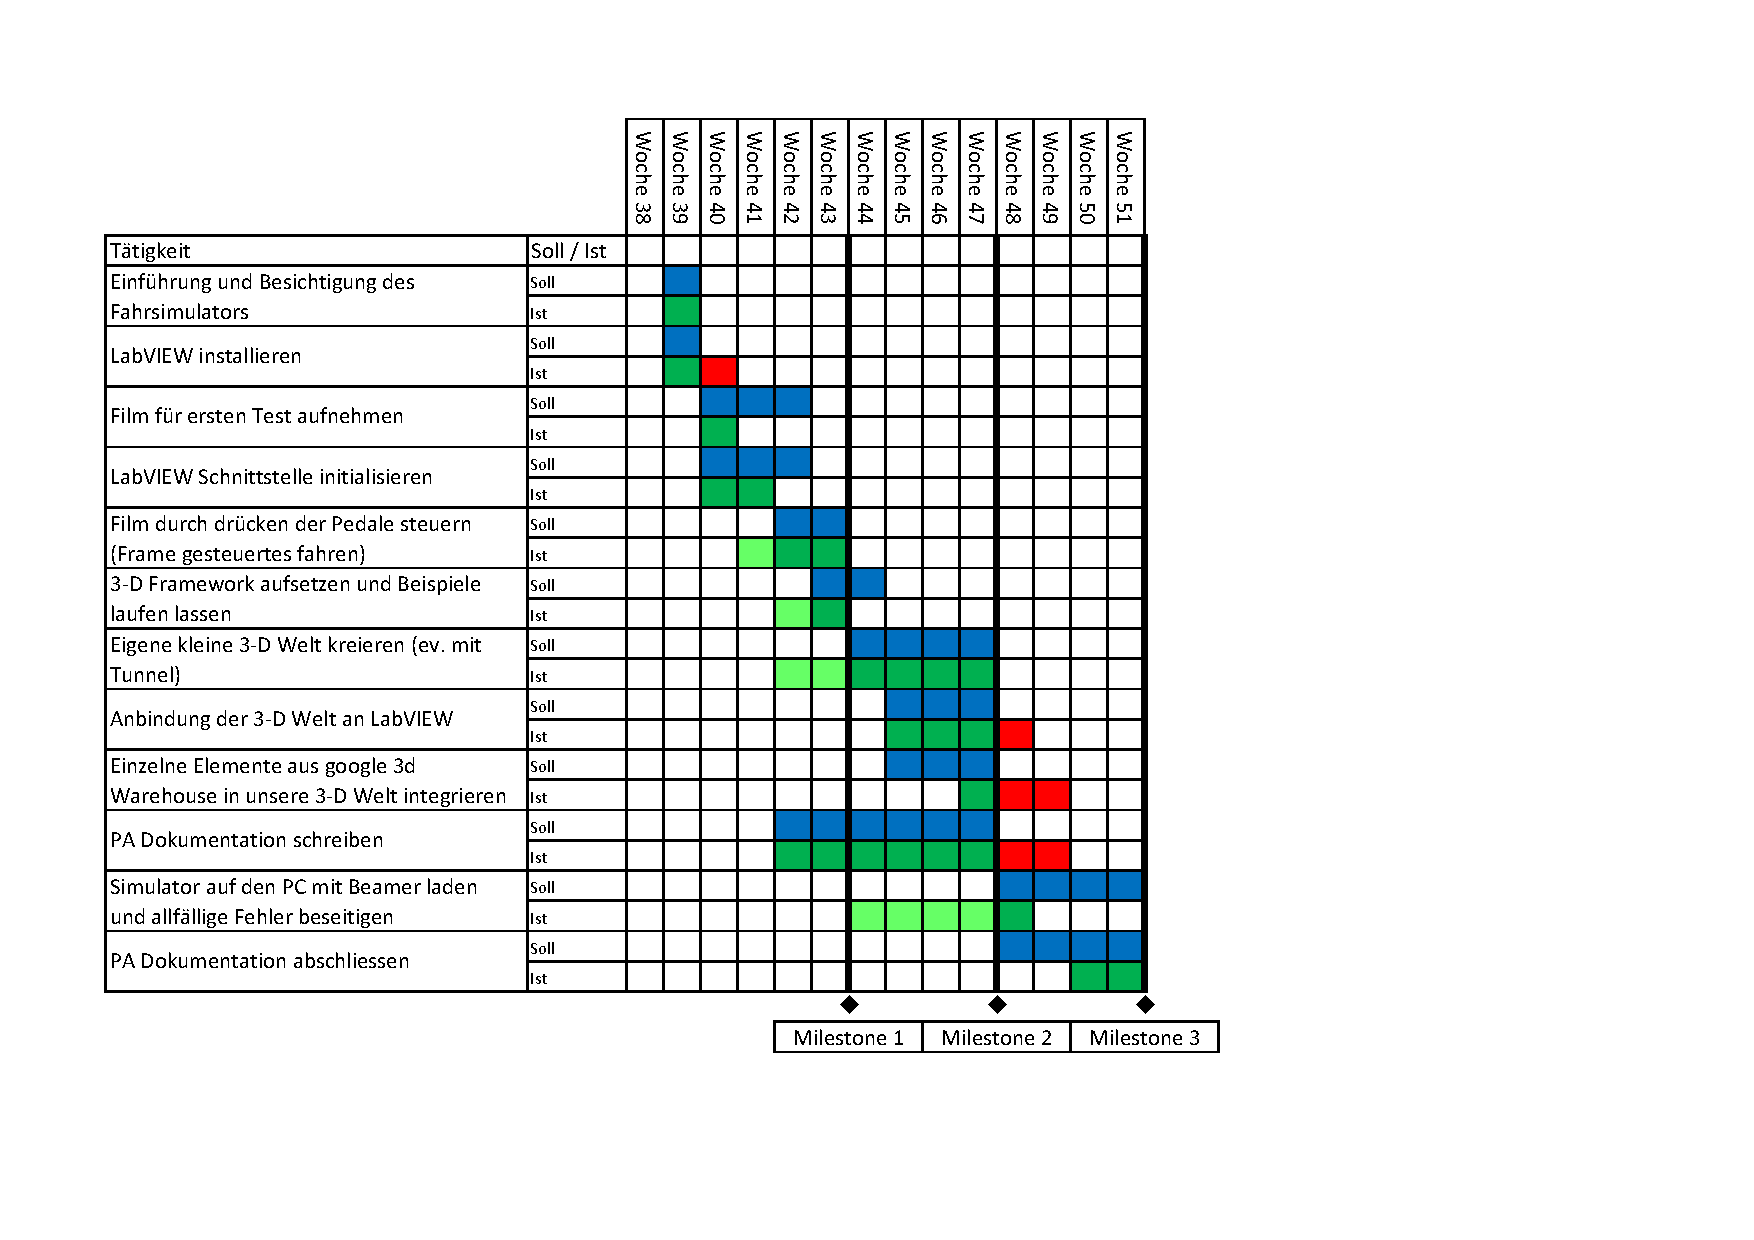
\includegraphics[width=1.0\linewidth]{src/Zeitplan.pdf}
\caption{Detailierter Zeitplan} % Titel der Grafik
\label{zeitplan} % Labelname
\end{figure}
\minisec{Einführung und Besichtigung des Fahrsimulators}
Der Aufbau des Fahrimulators und die Softwareumgebung wird besichtigt. Da das Projekt für die ETH durchgeführt wird, werden die Verantowrtlichen vorgestellt und mit ihnen Ziele und Anforderungen an die Arbeit besprochen. 
\minisec{LabVIEW installieren}
Das LabVIEW Programm wird auf unseren privaten Rechnern installiert. Wir machen uns damit vertraut können es für die Arbeit verwenden. 
\minisec{Film für ersten Test aufnehmen}
Um einen ersten Test mit einem Video-Player machen zu können wird ein geeignetes Video benötigt. Das Video zeigt Aufnahmen von einer Autofahrt und beinhaltet vorzugsweise eine Tunneleinfahrt.
\minisec{LabVIEW Schnittstelle initialisieren}
Im LabVIEW wird eine Schnittstelle eingerichtet um, die Werte des Cockpits in den Fahrsimulator zu übertragen. Entsprechend wird ein Gegenstück entwickelt um die Werte, die von LabVIEW gesendet werden, zu empfangen. 
\minisec{Film durch drücken der Pedale steuern (Frame gesteuertes fahren)}
Realisation eines Video Players, der einen Film abspielt. Die Abspielgeschwindigkeit wird durch das Drücken des Gas- oder Bremspedals im Cockpit beeinflusst. Beim drücken des Gaspedals wird der Film schneller und beim Bremspedal langsamer. 
\minisec{3D-Framework aufsetzen und Beispiele laufen lassen}
Für die Entwicklung des Fahrsimulators wird ein 3D Framework mit dem Namen OGRE verwendet. Dies soll in diesem Arbeitsschritt aufgesetzt, konfiguriert und getestet werden. Nach erfolgreichem Testen wird eine kurze einfache Szenen, die nur eine gerade Strasse enthält, erstellt. Die Szene wird aus dem Blickwinkel des Fahrers oder aus der Vogelperspektive gesehen. Zu Testzwecken soll das Fahrzeug mit den Pfeiltasten der Tastatur gesteuert werden.
\minisec{Eigene kleine 3-D Weld kreieren (ev. mit Tunnel)}
Es wird eine eigene 3-D Welt kreiert. Diese Szene kann bereits ein Tunnel enthalten. 
\minisec{Anbindung der 3-D Welt an LabVIEW}
In diesem Arbeitsschritt werden die LabVIEW Schnittstelle und die 3-D Welt zusammengefügt. Danach ist es möglich, das Fahrzeug in der Simulation durch Manipulation im Cockpit zu steuern. 
\minisec{Einzelne Elemente aus Google 3D Warehouse in unsere 3-D Welt integrieren}
Es werden Objekte aus dem Google 3D Warehous in die 3-D Welt integriert, um die Umgebung noch realistischer zu gestalten. 
\minisec{Dokumentation schreiben}
Mit der Dokumentation wird in der zweiten Hälfte der zur Verfügung stehenden Zeit begonnen. Die Besprechungen mit dem ETH Team oder den internen Betreuern werden von Beginn an protokolliert.
\minisec{Simulator auf den PC mit Beamer laden und allfällige Fehler beseitigen}
Der getestete Fahrsimulator wird definitiv auf den Rechner geladen und getestet. Kleinere Fehler und Unschönheiten werden noch beseitigt. 
\minisec{Dokumentation abschliessen}
Die Dokumentation wird von mehreren Personen gegengelesen, korrigiert und die definitive Version dann ausgedruckt und abgegeben. 